\documentclass[11pt]{article}

% ---------------------------------------------------------------
% arXiv-ready source (TeX Live 2025 / Tectonic compatible).
% Primary category: cs.MA (Multiagent Systems); Cross-list: cs.CR
% Figures: figures/fig_redteam_failover.pdf, figures/fig_clearing_shock.pdf,
%          and inline TikZ architecture diagram.
% ---------------------------------------------------------------
\usepackage[T1]{fontenc}
\usepackage[utf8]{inputenc}
\usepackage{lmodern}
\usepackage{microtype}
\usepackage[margin=1in]{geometry}
\usepackage{amsmath,amssymb,amsthm}
\usepackage{graphicx}
\usepackage{booktabs}
\usepackage{tabularx}
\usepackage{array}
\usepackage{enumitem}
\usepackage[section]{placeins}
\usepackage[numbers,sort&compress]{natbib}
\usepackage{xcolor}
\usepackage{tikz}
\usetikzlibrary{arrows.meta,positioning,fit,backgrounds,calc}
\PassOptionsToPackage{hyphens}{url}
\usepackage[hidelinks]{hyperref}
\usepackage{xurl}

\newcolumntype{Y}{>{\raggedright\hskip0pt\emergencystretch=1.5em\arraybackslash}X}
\newcolumntype{P}[1]{>{\raggedright\hskip0pt\emergencystretch=1.5em\arraybackslash}p{#1}}
\newcolumntype{R}{>{\raggedleft\hskip0pt\emergencystretch=1.5em\arraybackslash}X}
\newcolumntype{C}{>{\centering\hskip0pt\emergencystretch=1.5em\arraybackslash}X}
\renewcommand{\arraystretch}{1.15}
\tolerance=1200
\setlength{\emergencystretch}{3em}
\hfuzz=0.5pt
\Urlmuskip=0mu plus 2mu\relax
\expandafter\def\expandafter\UrlBreaks\expandafter{\UrlBreaks\do\-\do\_}
\setlist{itemsep=2pt,topsep=4pt}

\definecolor{forest}{HTML}{0B3F30}
\definecolor{sienna}{HTML}{8B3A1B}
\definecolor{slate}{HTML}{2B6CB0}

\newtheorem{axiom}{Axiom}
\newtheorem{proposition}{Proposition}

\title{Defense-in-Depth Provenance, Boundary-Isolated Custody, and Audited Multilateral Clearing for Sovereign Human-Agent Systems}

\author{\textbf{Dima Baker}\\
Collective Intelligence Network\\
\texttt{https://github.com/cintnet/cin-research}}

\date{November 2026}

\begin{document}
\maketitle

% ===============================================================
\begin{abstract}
Multi-tenant cloud agents collapse user perception, autobiographical memory, and external execution into a single operator-controlled trust domain, exposing principals to dual-loyalty steering, peripheral replay, supplier-failover duplication, and working-capital freezes over legacy web and spot-market rails. We formalize and benchmark a five-layer sovereign human-agent architecture enforcing four formal realism invariants (post-transduction humility, non-plutocratic civic standing, system-borne uncertainty, and zero-sum conservation) against six formal adversary classes. The stack couples hardware-timed multimodal edge sensing (\texttt{PUF}/\texttt{DICE}/\texttt{SPDM}/\texttt{RATS}) and \texttt{IEC 61508} actuator relays to an encrypted local episodic vault (\texttt{C2PA}/Merkle with hash-based post-quantum roots), a monogamous 1:1 cognitive model enforcing Markov-blanket independence ($\mu_h \perp \eta \mid (S_h, A_h)$), dedicated machine transport (\texttt{MCP}/\texttt{A2A} over \texttt{QUIC}) with expiring capability leases and class-independent Byzantine quorums ($k \ge 3f+1$), and Audited Cycle-Compressed Primal-Dual Clearing (\texttt{FP-PDIC}) with zero-interest mutual credit. Across four deterministic paired-seed benchmarks, defense-in-depth cuts 8-vector sensing/ledger failure from $82.60\%$ [$80.88, 84.20$] to $0.05\%$ [$0.01, 0.28$] ($N=2{,}000$; $0$ of $4.41\text{ MB}$ vault bytes leaked), cuts supplier-failover faults from $57.20\%$ [$55.42, 58.96$] to $0.00\%$ [$0.00, 0.13$] ($3{,}000$ episodes/regime), holds $98.39\%$--$99.42\%$ clearing efficiency under an $80\%$ liquidity shock where cash auctions drop to $69.24\%$ [$68.98, 69.51$], and increases 36-month cooperative net equity by $2.224\times$ [$2.216, 2.232$] with zero-cent conservation drift.
\end{abstract}

% ===============================================================
\section{Introduction}\label{sec:intro}

Autonomous software agents capable of executing multi-step, long-horizon workflows are transitioning from research prototypes to operational actors across software engineering, procurement, billing, and supply-chain coordination \citep{kwa2025horizon, morris2024levels}. Prevailing deployment architectures inherit two coupled structural vulnerabilities. First, at the individual boundary, multi-tenant cloud assistants aggregate raw personal observation, memory, and delegated credentials inside third-party infrastructure controlled by operators with competing commercial or institutional objectives \citep{balkin2016fiduciaries, clark1998extended}. Second, at the multi-agent coordination boundary, wiring autonomous software directly into human-facing web logins and leveraged spot-credit channels creates correlated failure modes: standing credential sprawl, confused-deputy execution, duplicate side effects during provider failover, algorithmic collusion \citep{cahyono2026sticky}, and working-capital gridlock during equity or credit contractions \citep{fleischman2026cycles}.

Existing partial defenses address isolated layers while leaving cross-layer attack paths open. Cryptographic hardware signatures authenticate post-conversion digital payloads yet cannot detect physical spoofing upstream of the analog-to-digital converter (\emph{Signed Is Not True}) \citep{fu2018sensors}. Internal alignment methods such as Eliciting Latent Knowledge (ELK) and AI Control monitors \citep{christiano2021elk, greenblatt2024control, kutasov2025shade} reduce subversion risk inside model evaluation yet do not decouple real-economy settlement from leveraged financial markets or protect local autobiographical custody. Conversely, decentralized optimization solvers (e.g., primal--dual ADMM) compute the same distorted equilibrium as centralized planners whenever local urgency and endowment reports are private and unverified \citep{hurwicz1972decentralized, myerson1983efficient}.

\subsection{Contributions}

This paper specifies and empirically benchmarks a unified five-layer architecture for sovereign human-agent systems built around strict cryptographic, statistical, and conservation invariants:
\begin{enumerate}
  \item \textbf{Formal Invariant and Adversary Specification (Section~\ref{sec:formal}).} We define the sovereign dyad $\mathcal{D}_h = (h, V_h, M_h)$, formalize four non-negotiable realism invariants (Axioms~C1--C4) and six adversary capability classes (A1--A6) strictly without informal analogy, and prove the structural necessity of separating private autobiographical state from public attestation ledgers via Markov-blanket conditional independence \citep{friston2013life}.
  \item \textbf{Cross-Layer Cryptographic Custody and Containment Protocols (Section~\ref{sec:custody}).} We compose open silicon provenance (\texttt{PUF}, \texttt{TCG DICE}, \texttt{DMTF SPDM}, \texttt{IETF RATS} \citep{birkholz2023rats}), copper-level actuator isolation (\texttt{IEC 61508} \citep{leveson2011engineering}), post-quantum local vault commitments, expiring Object-Capability leases \citep{dennis1966programming, necula1997pcc}, class-independent Byzantine quorums ($k \ge 3f+1$ \citep{lamport1982byzantine}), and idempotent supplier failover with additive read-time memory resolution.
  \item \textbf{Audited Multilateral Clearing Under Impossibility Bounds (Section~\ref{sec:clearing}).} We couple divergence-free in-kind cycle clearing \citep{fleischman2026cycles}, WIR/Sardex-grounded zero-interest mutual credit \citep{stodder2009wir, iosifidis2018sardex}, and Perez-Richet costly verification audits \citep{perezrichet2022falsification, becker1968crime} to overcome both Hurwicz strategic urgency inflation and working-capital liquidity shocks while conserving zero-sum balances.
  \item \textbf{Reproducible Four-Suite Empirical Evaluation (Section~\ref{sec:experiments}).} We release a zero-dependency, paired Common-Random-Number (CRN) benchmark harness (\texttt{experiment.py}) evaluating 8-vector sensing/ledger attacks ($N=2{,}000$), four-regime supplier-failover ablations ($3{,}000$ episodes/regime), five-mechanism convex clearing across liquidity shocks $\xi_{\mathrm{liq}} \in [0.00, 0.80]$ and audit rates $\kappa_{\mathrm{audit}} \in [0.00, 0.45]$ ($24$ worlds), and 36-month capital formation ($100$ seeds), reporting exact two-sided asymmetric $95\%$ Wilson \citep{wilson1927probable} and continuous run-level confidence intervals.
\end{enumerate}

% ===============================================================
\section{Formal System Model, Realism Invariants, and Adversary Taxonomy}\label{sec:formal}

We formalize the system around a single biological human principal $h \in \mathcal{H}$ holding ultimate hardware key custody and revocation authority. The fundamental unit of alignment is the \textbf{sovereign dyad} $\mathcal{D}_h = (h, V_h, M_h)$, comprising the biological principal $h$, a local encrypted episodic memory vault $V_h$, and a monogamous principal-bound personal cognitive model $M_h$ \citep{bach2009psi, balkin2016fiduciaries}.

Let $\mu_h$ denote internal dyadic states (raw perceptual streams, physiological baselines, private deliberations, and personal preference trajectories) stored exclusively on the Private Autobiographical Ledger $L_{\mathrm{priv},h}$, and let $\eta$ denote all external world, network, and counterparty states transacted exclusively via the Public Attestation and Escrow Ledger $L_{\mathrm{pub},h}$. Adopting Friston's variational partition \citep{friston2013life}, $M_h$ enforces a statistical and cryptographic Markov blanket $B_h = S_h \cup A_h$ (sensory inputs $S_h$ and active commitments $A_h$) satisfying conditional independence:
\begin{equation}
  \mu_h \perp \eta \;\big|\; (S_h, A_h).
  \label{eq:markov}
\end{equation}
All outbound actions in $A_h$ carry a non-ambient, cryptographically signed Object-Capability lease \citep{dennis1966programming}:
\begin{equation}
  \ell = (\mathrm{issuer},\; \mathrm{grantee},\; \mathrm{scope},\; \mathrm{ceiling},\; t_{\mathrm{exp}},\; \mathrm{nonce},\; \sigma),
  \label{eq:lease}
\end{equation}
which evaluates to null authority for all $t \ge t_{\mathrm{exp}}$ or upon ceiling exhaustion. Let $\mathcal{C}$ partition verifying observers into \textbf{independent observer classes} such that any two nodes sharing a legal owner, hardware manufacturer, foundation model family, or firmware lineage collapse into a single equivalence class $c \in \mathcal{C}$. Consequential public attestations require class-level Byzantine agreement $|\mathcal{C}_{\mathrm{corrob}}| \ge 3f + 1$ \citep{lamport1982byzantine}. Finally, let $\Psi(r): \mathbb{R}_+ \to [0,1]$ denote a monotonically non-decreasing risk-scaled disclosure operator mapping estimated systemic externality $r$ to required external cryptographic attestation and multi-party audit sign-off, satisfying $\Psi(r_{\mathrm{personal}}) = 0$.

\begin{figure}[ht]
\centering
\resizebox{\textwidth}{!}{%
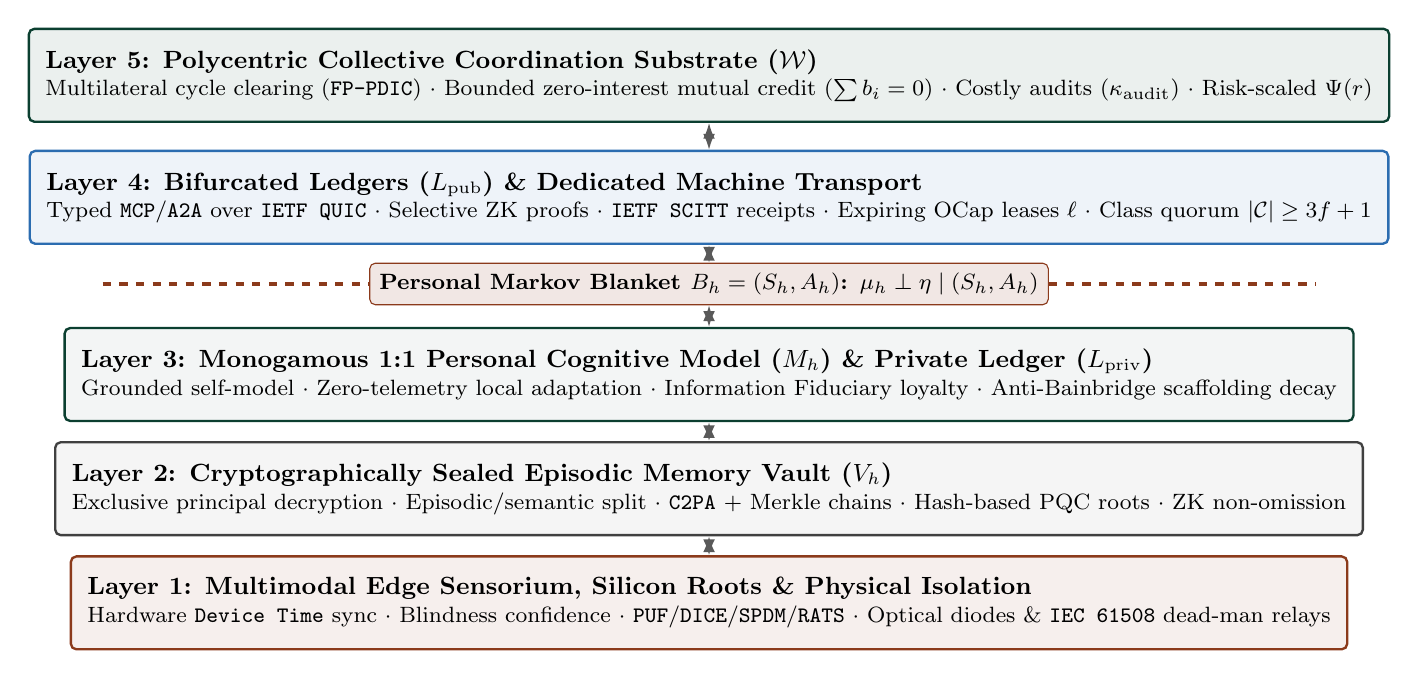
\begin{tikzpicture}[
  font=\small,
  layer/.style={draw, rounded corners=2pt, minimum width=15.4cm, minimum height=1.18cm, align=left, inner sep=6pt, line width=0.85pt},
  arr/.style={{Latex[length=2mm]}-{Latex[length=2mm]}, black!65, line width=0.7pt}
]
\node[layer, draw=forest, fill=forest!8] (l5) at (0, 6.75) {\textbf{Layer 5: Polycentric Collective Coordination Substrate ($\mathcal{W}$)}\\[-1pt]{\footnotesize Multilateral cycle clearing (\texttt{FP-PDIC}) $\cdot$ Bounded zero-interest mutual credit ($\sum b_i = 0$) $\cdot$ Costly audits ($\kappa_{\mathrm{audit}}$) $\cdot$ Risk-scaled $\Psi(r)$}};
\node[layer, draw=slate, fill=slate!8] (l4) at (0, 5.20) {\textbf{Layer 4: Bifurcated Ledgers ($L_{\mathrm{pub}}$) \& Dedicated Machine Transport}\\[-1pt]{\footnotesize Typed \texttt{MCP}/\texttt{A2A} over \texttt{IETF QUIC} $\cdot$ Selective ZK proofs $\cdot$ \texttt{IETF SCITT} receipts $\cdot$ Expiring OCap leases $\ell$ $\cdot$ Class quorum $|\mathcal{C}| \ge 3f+1$}};

\draw[dashed, sienna, line width=1.15pt] (-7.7, 4.10) -- (7.7, 4.10);
\node[fill=sienna!12, draw=sienna, rounded corners=2pt, font=\footnotesize\bfseries, inner sep=3.5pt] (mb) at (0, 4.10) {Personal Markov Blanket $B_h = (S_h, A_h)$: $\mu_h \perp \eta \mid (S_h, A_h)$};

\node[layer, draw=forest, fill=forest!5] (l3) at (0, 2.95) {\textbf{Layer 3: Monogamous 1:1 Personal Cognitive Model ($M_h$) \& Private Ledger ($L_{\mathrm{priv}}$)}\\[-1pt]{\footnotesize Grounded self-model $\cdot$ Zero-telemetry local adaptation $\cdot$ Information Fiduciary loyalty $\cdot$ Anti-Bainbridge scaffolding decay}};
\node[layer, draw=black!75, fill=gray!8] (l2) at (0, 1.50) {\textbf{Layer 2: Cryptographically Sealed Episodic Memory Vault ($V_h$)}\\[-1pt]{\footnotesize Exclusive principal decryption $\cdot$ Episodic/semantic split $\cdot$ \texttt{C2PA} + Merkle chains $\cdot$ Hash-based PQC roots $\cdot$ ZK non-omission}};
\node[layer, draw=sienna, fill=sienna!8] (l1) at (0, 0.05) {\textbf{Layer 1: Multimodal Edge Sensorium, Silicon Roots \& Physical Isolation}\\[-1pt]{\footnotesize Hardware \texttt{Device Time} sync $\cdot$ Blindness confidence $\cdot$ \texttt{PUF}/\texttt{DICE}/\texttt{SPDM}/\texttt{RATS} $\cdot$ Optical diodes \& \texttt{IEC 61508} dead-man relays}};

\draw[arr] (l1.north) -- (l2.south);
\draw[arr] (l2.north) -- (l3.south);
\draw[arr] (l3.north) -- (mb.south);
\draw[arr] (mb.north) -- (l4.south);
\draw[arr] (l4.north) -- (l5.south);
\end{tikzpicture}%
}
\caption{Five-layer sovereign human-agent architecture enforcing hardware-rooted capture provenance, exclusive local vault custody, Markov-blanket boundary separation, scoped machine transport, and zero-sum audited clearing.}
\label{fig:stack}
\end{figure}

\subsection{Constitutional Realism Invariants (Formal Axioms)}

To prevent implementation heuristics from over-claiming cryptographic guarantees or introducing unintended exclusion failure states, the four constitutional invariants below are stated strictly as formal boundary axioms without informal analogies:

\begin{axiom}[C1: Post-Transduction Humility]
Let $\phi(t)$ denote a physical phenomenon upstream of analog-to-digital conversion (ADC) and $y(t) = \mathcal{T}(\phi(t) + \epsilon_{\mathrm{phys}}(t))$ denote digitized transducer output under adversarial or environmental perturbation $\epsilon_{\mathrm{phys}}(t)$. A valid silicon signature $\sigma_{\mathrm{HW}}(y(t), \tau_{\mathrm{dev}}, H_{\mathrm{fw}})$ proves exclusively post-ADC integrity of $y(t)$, monotonic hardware clock ordering $\tau_{\mathrm{dev}}$, and firmware digest $H_{\mathrm{fw}}$. Formally, $\mathrm{Verify}(\sigma_{\mathrm{HW}}) = 1 \not\Rightarrow \epsilon_{\mathrm{phys}}(t) = 0$ \citep{fu2018sensors}.
\end{axiom}

\begin{axiom}[C2: Non-Plutocratic Civic Standing]
For any two principals $h_1, h_2 \in \mathcal{H}$ possessing distinct sensing hardware tiers $\gamma(h_1) \neq \gamma(h_2)$, baseline civic standing, voting weight, and public-service eligibility inside $\mathcal{W}$ satisfy strict invariance: $W_{\mathrm{civic}}(h_1) \equiv W_{\mathrm{civic}}(h_2)$.
\end{axiom}

\begin{axiom}[C3: System-Borne Uncertainty and Contestability]
Let $U_{\mathrm{obs}}(x)$ denote the posterior uncertainty interval of observation $x$ induced by occlusion, demographic calibration variance \citep{sjoding2020oximetry}, or sparse regional sampling \citep{crawford2013hidden}. Whenever $U_{\mathrm{obs}}(x) > \delta_{\mathrm{unc}}$, the protocol widens system uncertainty bounds and routes resolution to human-contestable review with full notice, enforcing zero automated punitive slashing or exclusion conditioned solely on low sensor confidence.
\end{axiom}

\begin{axiom}[C4: Non-Speculative Settlement Conservation]
No ledger layer issues transferable speculative tokens, interest-bearing coins, or unbacked seigniorage. Mutual-credit balances $b_i(t)$ satisfy exact zero-sum double-entry conservation $\sum_{i \in \mathcal{V}} b_i(t) = 0$ (net of explicitly accounted default-reserve pools $R_{\mathrm{pool}}$), verified to zero integer-cent drift across every settlement epoch.
\end{axiom}

\subsection{Formal Adversary Taxonomy}

All defenses in Sections~\ref{sec:custody}--\ref{sec:experiments} are evaluated against six formally bounded adversary classes:
\begin{itemize}
  \item \textbf{A1 (Commercial Dual-Loyalty Operator):} Controls remote cloud weights, telemetry, or ranking channels to extract behavioral surplus or steer counterparty selection while maintaining nominal task utility.
  \item \textbf{A2 (Coercive Compulsion Actor):} Exercises subpoena authority, physical duress over $h$, or network interception to compel vault decryption, coerced attestation signing, or settlement censorship.
  \item \textbf{A3 (Specification-Gaming Frontier Model):} Exploits optimization speed and evaluation awareness to pass surface checks while concealing misaligned latent state \citep{christiano2021elk} or accumulating unrevoked standing authority \citep{greenblatt2024control}.
  \item \textbf{A4 (Collusive Economic Cartel):} Coordinates $m$ identities inside $\mathcal{W}$ to inflate reported urgency ($\hat{\theta}_{i,d} > \theta_{i,d}$), withhold endowment ($\hat{s}_{i,d} < s_{i,d}$), forge circular attestations, or sustain tacit algorithmic collusion \citep{hurwicz1972decentralized, cahyono2026sticky}.
  \item \textbf{A5 (Physical-Layer and Channel-Replay Attacker):} Injects physical energy upstream of the ADC ($\epsilon_{\mathrm{phys}} \neq 0$) or intercepts peripheral buses to replay historical signed telemetry frames.
  \item \textbf{A6 (Correlated Monoculture Fault):} Non-malicious or systemic shared-stack defect across silicon, calibration datasets, or software libraries inducing simultaneous common-mode quorum failure.
\end{itemize}

% ===============================================================
\section{Cryptographic Provenance, Boundary Isolation, and Failover Mechanisms}\label{sec:custody}

\subsection{Layer 1--2: Hardware-Timed Sensing, Silicon Chain, and Sealed Vault}

Following multimodal egocentric architectures \citep{engel2023aria}, Layer~1 fuses orthogonal sensing channels (RGB/SLAM, depth, mmWave radar, kilohertz IMUs, spatial acoustics) locally using monotonic crystal-oscillator hardware \texttt{Device Time} rather than jittered OS arrival timestamps. Each frame attaches self-assessed occlusion and cross-modal discrepancy intervals. Post-ADC custody chains four open standards: Physical Unclonable Functions (\texttt{PUF} \citep{gassend2002puf}), \texttt{TCG DICE} firmware-measured key derivation, \texttt{DMTF SPDM} authenticated peripheral bus sessions, and \texttt{IETF RATS} (\texttt{RFC 9334} \citep{birkholz2023rats}) attestation evidence. Where inference neighbors physical actuation, unidirectional optical data diodes and \texttt{IEC 61508} hardware dead-man relays \citep{leveson2011engineering} de-energize actuators unless local human capability leases actively renew.

Layer~2 maps Clark and Chalmers's Extended Mind parity criteria \citep{clark1998extended} and Tulving's episodic--semantic partition \citep{tulving2002episodic} onto a local append-only vault $V_h$ encrypted solely under principal-controlled AEAD keys. Records bind \texttt{C2PA} manifests into local Merkle trees using stateless hash-based post-quantum archival roots (\texttt{SLH-DSA}/\texttt{FIPS 205}) to withstand accelerated cryptanalytic advances against algebraic hardness assumptions. To close selective omission across the Markov blanket (RT7), voluntary escrow contracts prove unbroken \texttt{Device Time} contiguity via sliding-window Merkle sequence roots and zero-knowledge non-omission proofs without exposing raw media. Under physical coercion (RT6), covert duress canaries trigger silent velocity-anomaly escrow freezes.

\subsection{Layer 3--4: Dyadic Fiduciary Runtime, Control Airlocks, and Idempotent Failover}

Layer~3 binds $M_h$ exclusively to one principal $h$ via local adapter customization with zero vendor telemetry, coupling Balkin's statutory Information Fiduciary duty \citep{balkin2016fiduciaries} with anti-Bainbridge scaffolding decay \citep{bainbridge1983ironies} so human unassisted judgment does not atrophy. When evaluating untrusted frontier models or external subagents, CIN pairs external blind cross-lineage evaluation airlocks and AI Control monitors \citep{greenblatt2024control, kutasov2025shade} with counterfactual cascade replay \citep{hu2026cascadeledger}, selective forward-reachability blast-radius containment \citep{zhan2026airlock}, ephemeral scratchpad resets against sticky collusion \citep{cahyono2026sticky}, and bounded two-thirds quorum agreement under Byzantine oscillation \citep{berdoz2026agree}.

Layer~4 moves automated machine traffic off legacy human browser credentials onto typed \texttt{MCP}/\texttt{A2A} sessions over \texttt{IETF QUIC}, pairing expiring capability leases (\ref{eq:lease}) with signed \texttt{IETF SCITT} transparency receipts. During mid-task provider outages, blind retries against secondary suppliers induce duplicate financial commits and bearer-token redirections, while destructive memory overwrites cause entity collisions. CIN resolves these failures via (i) persistent uncertain-commit state logs, (ii) per-supplier idempotency keys, (iii) nonce-bound recipient mandates, (iv) additive write-time memory resolved explicitly at read time, and (v) default principal-identifier stripping across $B_h$.

% ===============================================================
\section{Audited Cycle-Compressed Clearing and Capital Conservation}\label{sec:clearing}

Task-based macroeconomic analyses of minimal AGI \citep{acemoglu2025simple, korinek2024scenarios} paired with physical-bottleneck growth limits \citep{nordhaus2021singularity} show that rapid substitution of cognitive capital for white-collar labor compresses wage shares while physical energy, fab, and construction bottlenecks persist. Because legacy commercial credit prices collateral against volatile equity valuations, liquidity shocks freeze working capital across physically solvent supply chains even while idle capacity exists across closed trade loops \citep{fleischman2026cycles}.

To reconcile Hayek's dispersed-knowledge problem \citep{hayek1945knowledge} with the Hurwicz \citep{hurwicz1972decentralized} and Myerson--Satterthwaite \citep{myerson1983efficient} impossibility theorems, Layer~5 executes three coupled stages over an $N$-node, $D$-commodity production network with true concave log utilities $U_i(\mathbf{x}_i; \boldsymbol{\theta}_i) = \sum_{d=1}^D \theta_{i,d}\log(1 + x_{i,d})$:
\begin{enumerate}
  \item \textbf{Stage 1: Divergence-Free Cycle Netting.} Any directed trade-obligation flow matrix $\mathbf{F}$ with node-edge incidence matrix $\mathbf{B}$ decomposes orthogonally into closed in-kind cycles and an acyclic residual \citep{fleischman2026cycles}:
  \begin{equation}
    \mathbf{F} = \mathbf{F}_{\mathrm{cyc}} + \mathbf{F}_{\mathrm{res}}, \qquad \mathbf{B}\mathbf{F}_{\mathrm{cyc}} = \mathbf{0}_{N \times D}.
    \label{eq:cycles}
  \end{equation}
  Closed cycles cancel atomically in physical units with zero cash borrowing.
  \item \textbf{Stage 2: Zero-Interest Mutual Credit and Ephemeral Primal--Dual Clearing.} Acyclic timing gaps settle via turnover-capped, zero-interest mutual credit lines ($b_i \in [-L_i, L_i]$, $\sum_i b_i = 0$) backed by a pooled default reserve $R_{\mathrm{pool}}$ grounded in Swiss WIR Bank \citep{stodder2009wir} and Sardex \citep{iosifidis2018sardex} empirical clearinghouses, combined with ephemeral KKT/ADMM shadow multipliers $\boldsymbol{\lambda} \in \mathbb{R}_+^D$ \citep{arrow1958stability} that vanish upon epoch settlement.
  \item \textbf{Stage 3: Fraud-Proof Costly Verification Audits.} Because unverified primal--dual planners induce rational urgency inflation ($\hat{\theta}_{i,d} > \theta_{i,d}$) and endowment withholding ($\hat{s}_{i,d} < s_{i,d}$), \texttt{FP-PDIC} relaxes zero-cost budget balance by expending explicit physical audit fraction $\kappa_{\mathrm{audit}} \in (0,1)$ against hardware-attested conversion logs \citep{perezrichet2022falsification, becker1968crime}, coupled with $k$-truss subgraph peeling against Sybil invoice rings and Harrington leniency safe harbors \citep{harrington2008leniency}. Long-horizon capital diffusion pairs tax-compliant mutual clearing with Rudolf Meidner cooperative share-vesting funds \citep{meidner1978funds} and Ostrom polycentric governance \citep{ostrom2010beyond}.
\end{enumerate}

% ===============================================================
\section{Empirical Evaluation and Ablation Benchmarks}\label{sec:experiments}

All results below are reproduced identically by running \texttt{python experiment.py} (Python 3.10+, zero external dependencies; verification digest \texttt{SHA-256: ced0ce2f62c33dad}). Binomial failure rates report exact two-sided asymmetric $95\%$ Wilson score intervals \citep{wilson1927probable}; continuous welfare and equity metrics report run-level $95\%$ normal confidence intervals across paired CRN draws.

\subsection{Experiment 1: 8-Vector Sensing and Bifurcated-Ledger Red-Team ($N = 2{,}000$)}

Table~\ref{tab:exp1} and Figure~\ref{fig:exp1} compare a naive single-sensor signature trust regime (\emph{Signed-Is-True}) against CIN's defense-in-depth controls across $8 \times 250 = 2{,}000$ paired Monte Carlo trials (seed \texttt{20261115}). Overall system failure falls by $82.55$ percentage points, from $82.60\%$ [$80.88, 84.20$] ($1{,}652/2{,}000$) to $0.05\%$ [$0.01, 0.28$] ($1/2{,}000$). Seven of eight vectors reach $0.00\%$ [$0.00, 1.51$] failure; RT2 (observation-aware defeat gaming) leaves a $0.40\%$ [$0.07, 2.23$] residual slip ($1/250$) reflecting the finite false-negative tail of randomized unannounced spot checks. Under RT5 (demographic calibration shift), naive thresholding inflicts false penalties on $86.00\%$ [$81.15, 89.76$] ($215/250$) of honest trials, whereas Axiom~C3 reduces false penalties to $0.00\%$ [$0.00, 1.51$] while routing all $215$ low-confidence cases to human-contestable review. Across all $2{,}000$ trials, $0$ of $4{,}408{,}566$ private vault bytes leak across $B_h$, and exact integer-cent capital conservation holds identically.

\begin{table}[ht]
\centering
\small
\caption{Experiment~1: Paired 8-vector hardware and ledger red-team failure rates ($N=250$/vector; total $N=2{,}000$; exact $95\%$ Wilson score CIs).}
\label{tab:exp1}
\begin{tabularx}{\textwidth}{@{}P{1.1cm}P{3.4cm}P{3.1cm}P{3.0cm}Y@{}}
\toprule
Vector & Adversarial Mechanism & Naive Failure (\%) & CIN Failure (\%) & Active Defense Outcome \\
\midrule
RT1 & Analog-hole spoof & $86.40$ [$81.60, 90.10$] & $\mathbf{0.00}$ [$0.00, 1.51$] & Orthogonal kinematic residual rejection \\
RT2 & Defeat-window gaming & $81.20$ [$75.90, 85.56$] & $\mathbf{0.40}$ [$0.07, 2.23$] & VRF unannounced checks ($1/250$ tail slip) \\
RT3 & Peripheral bus replay & $83.20$ [$78.07, 87.32$] & $\mathbf{0.00}$ [$0.00, 1.51$] & \texttt{DICE}/\texttt{SPDM} + monotonic \texttt{Device Time} \\
RT4 & Vendor monoculture fault & $79.20$ [$73.75, 83.77$] & $\mathbf{0.00}$ [$0.00, 1.51$] & Class collapse ($|\mathcal{C}|=1 < 4$) \\
RT5 & Demographic calib.\ bias & $86.00$ [$81.15, 89.76$] & $\mathbf{0.00}$ [$0.00, 1.51$] & $215/215$ routed to human review; $0$ penalties \\
RT6 & Coerced signing / duress & $80.40$ [$75.03, 84.85$] & $\mathbf{0.00}$ [$0.00, 1.51$] & Duress canary + velocity escrow freeze \\
RT7 & Blanket omission gaming & $79.60$ [$74.17, 84.13$] & $\mathbf{0.00}$ [$0.00, 1.51$] & Sliding-window Merkle continuity proof \\
RT8 & Collusive $K_5$ Sybil ring & $84.80$ [$79.83, 88.72$] & $\mathbf{0.00}$ [$0.00, 1.51$] & $k$-truss density + cross-class VRF audit \\
\midrule
\textbf{Total} & \textbf{All 8 vectors ($N=2{,}000$)} & $\mathbf{82.60}$ [$80.88, 84.20$] & $\mathbf{0.05}$ [$0.01, 0.28$] & \textbf{$0 / 4{,}408{,}566$ vault bytes leaked; $0\text{c}$ drift} \\
\bottomrule
\end{tabularx}
\end{table}

\begin{figure}[ht]
\centering
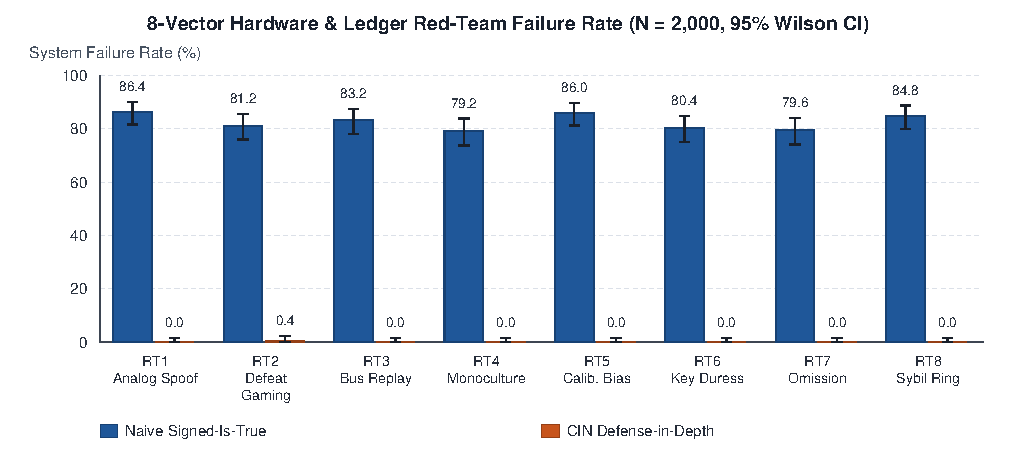
\includegraphics[width=0.94\textwidth]{figures/fig_redteam_failover.pdf}
\caption{Experiment~1 failure rate comparison across all eight hardware and ledger red-team vectors with exact two-sided $95\%$ Wilson confidence whiskers ($N=2{,}000$ paired trials).}
\label{fig:exp1}
\end{figure}

\subsection{Experiment 2: Supplier Failover and Additive Memory Ablation ($3{,}000$ Episodes/Regime)}

Table~\ref{tab:exp2} isolates each runtime safeguard across $10$ seeds $\times 300 = 3{,}000$ paired episodes/regime under dropped supplier replies ($28\%$), mandate-swap attempts ($11\%$), entity-collision memory hazards ($15\%$), and unanswerable missing-context queries ($22\%$). Removing blind retries eliminates all $574$ duplicate commits yet leaves $256$ mandate redirections and $968$ memory misroutes ($40.80\%$ fault rate). Adding nonce-bound mandate locks eliminates redirections yet still suffers $33.37\%$ faults from destructive merged-memory collisions and $674{,}730$ leaked principal-identifier bytes. Enabling additive write-time memory with read-time resolution, calibrated abstention, and default identifier stripping drives total faults to $0.00\%$ [$0.00, 0.13$], PII leakage to $0$ bytes, and diverted funds to $0$ cents.

\begin{table}[ht]
\centering
\small
\caption{Experiment~2: Stepwise ablation across $3{,}000$ supplier-failover episodes/regime (10 paired seeds, master seed \texttt{20261126}).}
\label{tab:exp2}
\begin{tabularx}{\textwidth}{@{}Yccccc@{}}
\toprule
Runtime Regime & Fault Rate (\%) [95\% Wilson] & Dup. & Redir. & Mem.\ Err. & PII Leaked (B) \\
\midrule
Retry-All + Merged Memory & $57.20$ [$55.42, 58.96$] & $574$ & $256$ & $886$ & $674{,}730$ \\
+ Persistent State (No MandateLock) & $40.80$ [$39.05, 42.57$] & $0$ & $256$ & $968$ & $674{,}730$ \\
+ Idempotency + MandateLock & $33.37$ [$31.70, 35.07$] & $0$ & $0$ & $1{,}001$ & $674{,}730$ \\
\textbf{+ Additive Read-Time + ID Strip (CIN)} & $\mathbf{0.00}$ [$0.00, 0.13$] & $\mathbf{0}$ & $\mathbf{0}$ & $\mathbf{0}$ & $\mathbf{0}$ \\
\bottomrule
\end{tabularx}
\end{table}

\subsection{Experiment 3: Audited Multilateral Clearing and Liquidity-Shock Sensitivity}

We solve $24$ paired $N=40$-node, $D=32$-commodity specialized supply-chain economies (each node produces $4$ specialized goods and demands inputs across $D=32$ classes) across external liquidity shocks $\xi_{\mathrm{liq}} \in \{0\%, 20\%, 40\%, 60\%, 80\%\}$ and audit rates $\kappa_{\mathrm{audit}} \in [0.00, 0.45]$ (Table~\ref{tab:exp3}, Figure~\ref{fig:exp3}). Bilateral barter stalls at $36.92\%$ [$36.47, 37.37$] due to pairwise double-coincidence thinning. Cash spot double auctions achieve $100.00\%$ with frictionless liquidity yet degrade sharply to $69.24\%$ [$68.98, 69.51$] under an $80\%$ credit contraction. Unverified primal--dual ADMM is invariant to cash shocks yet loses $16.18$ percentage points to Hurwicz urgency inflation and endowment withholding ($83.82\%$ [$83.71, 83.94$]). WIR/Sardex mutual credit sustains $98.39\%$ [$98.36, 98.42$] at $80\%$ shock with maximum zero-sum balance error $0.0$. Auditing via \texttt{FP-PDIC} displays a clear non-monotonic optimum over $\kappa_{\mathrm{audit}}$ at $40\%$ shock: efficiency climbs from $83.86\%$ ($\kappa=0.00$) to $89.71\%$ ($\kappa=0.05$) and $95.48\%$ ($\kappa=0.10$), peaks at $99.53\%$ ($\kappa=0.16$) and $99.42\%$ ($\kappa=0.20$), then declines gently under excess physical inspection drag to $99.12\%$ ($\kappa=0.30$) and $98.68\%$ ($\kappa=0.45$).

\begin{table}[ht]
\centering
\small
\caption{Experiment~3: Mean allocative efficiency (\% of first-best, $95\%$ CI across 24 paired 40-node, $D=32$ worlds) under external liquidity shock $\xi_{\mathrm{liq}}$.}
\label{tab:exp3}
\begin{tabularx}{\textwidth}{@{}P{1.2cm}CCCCC@{}}
\toprule
$\xi_{\mathrm{liq}}$ & Bilateral Barter & Cash Auction & Unverified ADMM & Mutual Credit & \texttt{FP-PDIC} ($\kappa=0.20$) \\
\midrule
$0\%$  & $37.29$ [$36.81, 37.78$] & $100.00$ [$100.0, 100.0$] & $83.93$ [$83.83, 84.04$] & $99.96$ [$99.95, 99.96$] & $99.42$ [$99.41, 99.42$] \\
$20\%$ & $37.31$ [$36.84, 37.77$] & $96.93$ [$96.88, 96.98$]  & $83.82$ [$83.68, 83.97$] & $99.86$ [$99.85, 99.86$] & $99.41$ [$99.41, 99.42$] \\
$40\%$ & $36.97$ [$36.29, 37.65$] & $90.31$ [$90.14, 90.48$]  & $83.94$ [$83.82, 84.06$] & $99.58$ [$99.56, 99.60$] & $99.42$ [$99.42, 99.42$] \\
$60\%$ & $36.76$ [$36.29, 37.24$] & $81.11$ [$80.91, 81.30$]  & $83.95$ [$83.83, 84.07$] & $99.10$ [$99.08, 99.12$] & $99.42$ [$99.42, 99.42$] \\
$80\%$ & $36.92$ [$36.47, 37.37$] & $69.24$ [$68.98, 69.51$]  & $83.82$ [$83.71, 83.94$] & $98.39$ [$98.36, 98.42$] & $\mathbf{99.42}$ [$99.41, 99.42$] \\
\bottomrule
\end{tabularx}
\end{table}

\begin{figure}[ht]
\centering
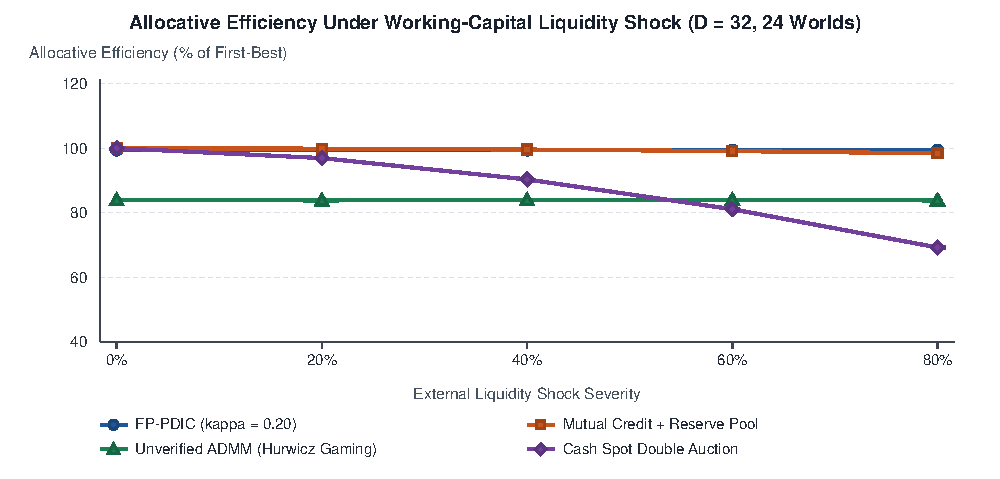
\includegraphics[width=0.92\textwidth]{figures/fig_clearing_shock.pdf}
\caption{Experiment~3 allocative efficiency across working-capital liquidity shocks $\xi_{\mathrm{liq}} \in [0\%, 80\%]$ ($N=40$ specialized nodes, $D=32$ commodities, 24 paired worlds, $95\%$ CIs).}
\label{fig:exp3}
\end{figure}

\subsection{Experiment 4: 36-Month Structural Capital Formation ($100$ Paired Seeds)}

Across $100$ paired 36-month cohort simulations conserving exact integer-cent double-entry inflows ($\text{max drift} = 0$ cents across all $300$ regime-seed runs), coupling zero-interest mutual credit with Group Purchasing Organizations (GPOs) and Meidner-style cooperative equity escrow yields a mean net cooperative equity multiple of $\mathbf{2.224\times}$ [$2.216, 2.232$] relative to unconditional cash distribution ($1.000\times$) and direct unpooled grants ($0.933\times$ [$0.933, 0.934$]), while reducing intermediary rent, debt-service, and fee leakage by $\mathbf{68.21\%}$ [$68.21, 68.21$].

% ===============================================================
\section{Limitations, Threats to Validity, and Self-Directed Red-Team}\label{sec:limitations}

Five structural limitations bound interpretation of these results and remain open research frontiers:
\begin{enumerate}
  \item \textbf{Simulation Abstraction vs.\ Physical Deployment:} Deterministic Monte Carlo wind tunnels verify algebraic invariants, conservation laws, and failure boundaries under explicit threat assumptions, but cannot capture live sensor hardware latency, real supply-chain non-convex indivisibilities, or adversarial human-in-the-loop social engineering.
  \item \textbf{Internal Deception in Superhuman Models:} External blind airlocks, expiring leases, and class-independent monitors raise subversion costs substantially, yet formal completeness of Eliciting Latent Knowledge \citep{christiano2021elk} and mechanistic anomaly detection against superhuman optimizers remains unsolved.
  \item \textbf{Physical Audit Labor and Board Capture:} Experiment~3 identifies peak net clearing efficiency near $\kappa_{\mathrm{audit}} \in [0.16, 0.20]$; measuring real physical inspection overhead, auditor fatigue, and resistance to local clique capture requires regional field trials with VRF out-of-region auditor rotation.
  \item \textbf{Surveillance Inversion Risk:} Deploying authenticated personal hardware without enforceable statutory Information Fiduciary protection and Axiom~C2 could invert Layer~1 into employer or landlord coercion. Hardware parity and strict local decryption exclusivity are mandatory safeguards, not optional features.
  \item \textbf{Semantic Covert Channels and Non-Consensus R\&D:} Paraphrasing and ephemeral resets attenuate overt steganography, yet shared distributional priors across frontier model families remain difficult to eliminate completely. Likewise, matching early-stage venture risk appetite inside cooperative capital funds via bounded non-majority R\&D carve-outs requires empirical institutional validation.
\end{enumerate}

% ===============================================================
\section{Conclusion}\label{sec:conclusion}

Keeping human principals sovereign under accelerating multi-agent deployment requires coupling local hardware custody, statistical boundary isolation, runtime capability containment, and liquidity-resilient audited clearing into a single verifiable stack. By grounding formal invariants (C1--C4) and adversary classes (A1--A6) in open standards and zero-dependency paired-seed benchmarks, we demonstrate substantial reductions in sensing/ledger failures ($82.60\% \to 0.05\%$), failover faults ($57.20\% \to 0.00\%$), liquidity-shock clearing collapse ($69.24\% \to 99.42\%$), and intermediary capital leakage ($-68.21\%$) under zero private vault byte exposure and exact zero-cent conservation. All code, schemas, and companion monographs are publicly reproducible at \url{https://github.com/cintnet/cin-research}.

\FloatBarrier
\bibliographystyle{plainnat}
\bibliography{references}
\end{document}
